  %%%%%%%%%%%%%%%%%%%%%%%%%%%%%%%%%%%%%%% -*- coding: utf-8; mode: latex -*- %%
  %
%%%%%                         CHAPTER
 %%%
  %

% $Id: 1020-lorem-ipsum.tex,v 1.2 2009/06/19 15:51:46 david Exp $
% $Log: 1020-lorem-ipsum.tex,v $
% Revision 1.2  2009/06/19 15:51:46  david
% *** empty log message ***
%
% Revision 1.1  2007/11/23 09:52:39  david
% *** empty log message ***
%
%

  %%%%%%%%%%%%%%%%%%%%%%%%%%%%%%%%%%%%%%%%%%%%%%%%%%%%%%%%%%%%%%%%%%%%%%%%%%%%%
  %
%%%%%                           HEAD MATTER
 %%%
  %

\chapter{Apache Hadoop}
%\addcontentsline{lof}{chapter}{\thechapter\quad Lorem Ipsum}
%\addcontentsline{lot}{chapter}{\thechapter\quad Lorem Ipsum}
\label{ch:hadoop}




  %%%%%%%%%%%%%%%%%%%%%%%%%%%%%%%%%%%%%%%%%%%%%%%%%%%%%%%%%%%%%%%%%%%%%%%%%%%%%
  %
%%%%%                        FIRST SECTION
 %%%
  %

\section{Introduction}

Apache Hadoop ~\cite{h17} is an open-source software framework for large-scale data
processing. It includes a distributed file system called the Hadoop Distributed
File System (HDFS) and a framework for MapReduce. Many data analysis,
data warehousing and machine learning solutions have been built on top of it.
The most commonly known extensions of Hadoop are Apache Pig ~\cite{21}, Apache
Hive ~\cite{22}, Apache HBase  ~\cite{26}, Apache Zookeeper  ~\cite{27} and Apache Mahout  ~\cite{23}.
Recent version of Hadoop also include a resource negotiator called Yet-Another-
Resource-Negotiator (YARN), often also referred to as NextGen MapReduce or
short MRv2. YARN is, inter alia, used to execute MapReduce jobs. The design
and concepts used by Hadoop are inspired by the Google papers about GFS and
MapReduce ~\cite[p.~9]{h17}. Similar to MapReduce on GFS, Hadoop is exploiting data
locality for MapReduce jobs by trying to execute map jobs on a DataNode which
hosts the data. If not possible, the framework will attempt to execute the job
on a node close to the location of data, for instance on the same rack. This can
greatly improve the overall performance [28] and reduces the network bandwidth
requirements.



  %%%%%%%%%%%%%%%%%%%%%%%%%%%%%%%%%%%%%%%%%%%%%%%%%%%%%%%%%%%%%%%%%%%%%%%%%%%%%
  %
%%%%%                      SECOND SECTION
 %%%
  %

\section{Hadoop File System(HDFS)}
 HDFS  is   Hadoop’s   distributed  file  system   which  has   been  designed  after  Google  File System.It was initially created to be used in a Map-Reduce computational framework of Hadoop by Apache though later on it started to be used for other big data applications as a storage which can support massive amount of data on commodity machines.Hadoop File System were intended to be distributed for being accessed and used inside by distributed processing machines of Hadoop with a short response time and maximum parallel streaming factor. On the other hand, in order for HDFS to be used as a storage of immutable data for applications like Facebook, the high availability is a key requirement besides the throughput and response time.Moreover, as a file system to be compliant to the common file system standard, it provides posix like interface in terms of operations, however it has a weaker consistency model than posix which is being discussed later on in this section.
 \subsection{HDFS Architecture}
HDFS  splits   up  each  file  into  smaller  blocks  and replicates  each block  on a different random
machine.  Machines   storing  replicas   of  the  blocks   called  DataNode. On the other hand since
it  needs   to  have  namespace  metadata  accessible  altogether,  there  is   a  dedicated metadata
machine  called  NameNode.  For  having  fast  access   to  metadata,  NameNode  stores
metadata  in  memory.  Accessing  to  HDFS  happens   through  its   clients,  each  client  asks
NameNode  about  namespace  information,  or  location  of  blocks   to  be  read  or  written, then it
connects   to  DataNodes   for  reading  or  writing  file  data.  Figure\ref{fig:HDFS_Architecture}  shows   the  deployment  of
different nodes in HDFS.
\begin{figure}[htb]
  \centering
 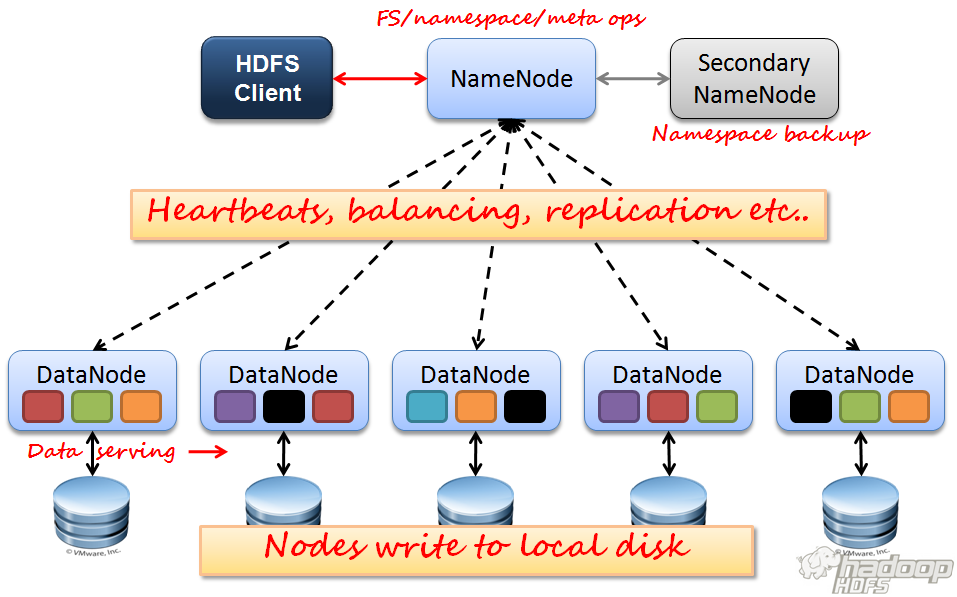
\includegraphics[scale=0.5]{figs/preliminar/HDFS_Architecture.png}
  \caption{HDFS Architecture.}
  \label{fig:HDFS_Architecture}
\end{figure}
\subsection{HDFS NameNode}
NameNode  is   known  as   metadata  server  of  HDFS. Its  multithreaded server in which size of
the  thread  pool  is   configurable.  It  keeps   all  metadata  information  in  memory   which  is
described  in  the  next  section.  The  way   NameNode  protects   race  condition  for  metadata
modification  is   based  on  read/write  lock.  It  splits   all  operations   into  read  or  write  operations.Its procedure is shown in alogithm \ref{NormalNameNode}.In this way multiple read operations could be run in parallel though they are serialized with
each single write operation.
Other  than  serving  client’s   requests,  NameNode  has   been  serving  part  for  DataNodes,  via
this   service. DataNodes  notice NameNode about receiving or deletion of blocks  or they  send
over  list  of  their  replicas   periodically.  Moreover,  NameNode  has   one  still running  thread
namely   ReplicationMonitor  to  get  under-replication  and  over-replication  under  its   radar  and
plans for deletion/replication accordingly.
Moreover,  LeaseMonitor  controls   the  time  limit  that  each  client  holds   the  write  operation  of files.  So  it  walks   through  all  leases   and  inspect  their  soft-limit/hard-limit  and  decides   to
recover or revoke an expired lease.

\begin{algorithm}[h]
\caption{System-Level locking schema in HDFS}
\label{NormalNameNode}
\begin{algorithmic}
\State \textbf{Operation } lock
\If { op.type = write }
\State ns.acquireWriteLock()
\Else
\State ns.acquireReadLock()
\EndIf\\
\State \textbf{Operation }  perform Task
 \State //Operation body \\
\State \textbf{Operation } unlock
\If { op.type = write }
\State ns.releaseWriteLock()
\Else
\State ns.releaseReadLock()
\EndIf
 

\end{algorithmic}
\end{algorithm}

\subsection{HDFS consistency model}
\begin{enumerate}
\item \textbf{FileSystem Operations}\\
In  general  most  of  the  distributed  file  systems   like  GFS  and  HDFS  have  a  relaxed
version  of  consistency   because  of  the  impossibility   result  of  CAP  theorem \cite{cap}
which  limits   scalability   of  file  system.  Even  though  some  works   refer  to  HDFS  as
sequential  consistent  file  system   for  data  and  from   filesystem   operations   point  of
view,  it  does   not  certainly   have  sequential  consistency   due  to  nonatomic   write
operation.  HDFS  serializes   read/write  operations  just at the primitive operations’ level
not  the  files   blockdata.  As  each write operations  consists  of multiple micro addBlock
operations   which  makes   it  unsortable  when  multiple  parallel  reads   are  being
performed with one write. Though it protects  multiple writes  by  means  of a persistable
mechanism called lease.
\item \textbf{Primitive NameNode Operations}\\
From   primitive  operations   point  of  view, HDFS is  strongly  consistent in both data and
metadata level.
From   data  level  it  is   strongly   consistent  because  each  file’s   block   is  not available for
read  unless   it  gets   completely   replicated.  It  means   write  operation  should  be
completely   finished  first,  then  readers   will  all  get  the  same  version  of  that  block   and
there is not case of version mismatch in the replicas read by two different readers.
From   metadata  level,  as   already   been  mentioned, system  level lock  serializes  all the
write  operations   which  results   in  mutated  state  of  all  writes   bing  available  for  all
readers.

\end{enumerate}

\subsection{POSIX compliant filesystem}
POSIXfs   is   file  system   part  of  POSIX  operating  system.  It  has   been  being  a  standard  for
designing  filesystems.  It  is   about  naming,  hardlinks,  access   control,  time  stamping  and
standard  folder  hierarchy.  Under  POSIX  standards,  almost  all  file  operations   shall  be
linearized.  Specifically   all  read  operations   should  have  effects   of  all  previous   write
operations.
HDFS  is   not  fully  POSIX compliant, because the requirements  for a POSIX file system  differ
from   the  target  goals   for  a  Hadoop  application.  The  tradeoff  of  not  having  a  fully
POSIXcompliant  file  system   is   increased  performance  for  data  throughput  and  support  for
nonPOSIX  operations   such  as   Append.  Moreover,  HDFS  consistency   model  is   weaker
than  POSIX.  HDFS  is   strongly   consistent  from   primitive  HDFS  operations   while  from
filesystem   operations   it  has   a  relaxed  version  of  consistency,  on  the  other  hand,  POSIX
filesystem operations are linearizable which is the highest level of consistency.

 %%%%%%%%%%%%%%%%%%%%%%%%%%%%%%%%%%%%%%%%%%%%%%%%%%%%%%%%%%%%%%%%%%%%%%%%%%%%%
  %
%%%%%                         ANOTHER SECTION
 %%%
  %


 

  %
 %%%
%%%%%                        THE END
  %
  %%%%%%%%%%%%%%%%%%%%%%%%%%%%%%%%%%%%%%%%%%%%%%%%%%%%%%%%%%%%%%%%%%%%%%%%%%%%%

%%% Local Variables: 
%%% mode: latex
%%% TeX-master: "tese"
%%% End: 
